\newcommand{\btheta}{\boldsymbol{\theta}}
\newcommand{\data}{\boldsymbol{D}}

\author[Lecturer1]{Brendon J. Brewer\\
Department of Statistics, The University of Auckland}

\chapter{Bayesian Inference How-To}

\section{Introduction}
Most scientific observations are not sufficient to give us definite answers
to all of our questions. It is rare that a theory is ever {\it totally}
ruled out by a dataset. Instead, the data makes some theories more plausible
and some less plausible. Bayesian inference is the tool we use to model this
reasoning process, and to make quantitative statements about how much
uncertainty we should have about our conclusions. This takes the mystery out
of data analysis, because we no longer have to come up with a new method
every time we face a new problem. Instead, we simply specify exactly what
information we are going to use, and then we compute the results.

%In previous chapters you've had an overview of the fundamental ideas
%of Bayesian inference along with its historical development. This chapter
%focuses on putting these ideas into practice.

Any particular application of Bayesian inference involves making choices
about what data you are analysing, what questions you are
trying to answer, and what assumptions you are willing to make.
In principle, it's usually best to work with your data in the most
raw form possible, although this is often too difficult in practice.
Therefore, most scientists work with data that has been processed (by a ``pipeline'') and reduced to manageable size. To do Bayesian inference, you
need to specify what {\it prior information} you have (or are willing to
assume) about the problem, in addition to the data. Prior information is
necessary: what you can learn from a data set depends on what you know, for
example, about how it was produced.

Once you have your data, and have specified your prior information as well,
you are faced with the question of how to calculate the
results. Usually you want to calculate the {\it posterior distribution} for some
unknown quantities (also known as ``parameters'') given your data,
and then present the results in an
understandable way. Since we are often dealing with complicated probability
distributions in high dimensional spaces, numerical methods are usually used.
The most popular and useful numerical techniques are the Markov Chain Monte
Carlo methods, often abbreviated as
MCMC\footnote{Some people claim that MCMC stands for
Monte Carlo Markov Chains, but they are wrong.}.
The rediscovery of MCMC in the 1990s
is one of the main reasons why Bayesian inference is so popular now.
While there were many strong philosophical arguments in favour of a Bayesian
approach before then, many people were still uncomfortable with the
subjective elements involved. However, once MCMC made it easy to compute the
consequences of Bayesian models more easily, people simply became more relaxed
about these subjective elements.

A huge variety of MCMC methods exists, and it would be
unwise to try to cover them all in this winter school. Therefore I will focus
on a small number of methods that are relatively simple to implement, yet quite powerful
and widely applicable. I will try to emphasise methods that are {\it general},
i.e. methods that will work okay on most problems you might encounter. One
disadvantage of this approach is that the methods we cover are not necessarily
the most efficient methods possible. If you're mostly interested in one
specific application, you'll probably be able to achieve better performance
by using a more sophisticated algorithm, or by taking advantage of the particular
properties of your problem.

There are many popular software packages (and many more unpopular ones)
available for doing Bayesian Inference, such as JAGS (Just Another Gibbs Sampler),
Stan, emcee, MultiNest, my own DNest3, and many more.
I won't be teaching you how to use any of these programs.
If you or your collaborators already use one of them, that's a great reason to
learn it! Please see the appendix for a discussion of the advantages and
disadvantages of these packages.

%JAGS is extremely convenient to use

\section{Python}
Due to its popularity and relatively shallow learning curve,
I will be using Python to implement the algorithms. The code I use will be
written so that it works in either Python 2 or 3. I will also assume that
each program has imported the following libraries:

\begin{minted}[mathescape,
               numbersep=5pt,
               gobble=2,
               frame=lines,
               framesep=2mm]{python}
  import numpy as np
  import numpy.random as rng
  import matplotlib.pyplot as plt
  import copy
\end{minted}

\section{Notation for Probability Distributions}
There are two main types of notation that are used in probability theory. The
first type is mathematically correct and conceptually
clear, yet results in equations that are very large, complicated,
and difficult to read.
The second type is a very compact notation which makes equations a lot
shorter and easier to read, but could be misinterpreted if you are not used to
it. I prefer the compact notation, but to prevent any misunderstandings
I'll describe both below.

Suppose we're about to flip a coin $N$ times, and are interested in the
quantity $X$, the number of times the result is heads. According
to the standard assumptions, the possible values for $X$ are the integers from 0
to 10, and the probability distribution for $X$ is given by
a binomial distribution:

\begin{eqnarray}
P(X = x) &=& \left(\begin{array}{cc}10\\ x\end{array}\right)
\left(\frac{1}{2}\right)^x\left(\frac{1}{2}\right)^{10 - x}\\
&=& \left(\begin{array}{cc}10\\ x\end{array}\right)
\left(\frac{1}{2}\right)^{10}
\end{eqnarray}
The equation gives us all the probabilities we want, i.e. $P(X=0)$, $P(X=1)$,
and so on. The lower case $x$ is a dummy variable: like the index in a sum, it
can be replaced by any other symbol and the equation still holds. For example,
replacing $x$ with $a$ gives:
\begin{eqnarray}
P(X = a) &=& \left(\begin{array}{cc}10\\ a\end{array}\right)
\left(\frac{1}{2}\right)^{10}.
\end{eqnarray}

The compact notation ignores all of this and simply writes $p(x)$ instead of
$P(X=x)$:
\begin{eqnarray}
p(x) &=& \left(\begin{array}{cc}10\\ x\end{array}\right)
\left(\frac{1}{2}\right)^{10}
\end{eqnarray}
Since $X$, the actual number of heads, isn't written anywhere, we forget it
exists and just use the lower case $x$ for that purpose, even though it was
originally a dummy variable!
The key to understanding this notation is to read $p(x)$ as ``the probability
distribution for $x$'', and to understand what the expression following it
really means. If the set of possible $x$ values is continuous (so $p(x)$ gives
the probability {\it density} instead of a probability itself) then the
notation doesn't change.

The compact notation is especially helpful in Bayesian statistics because
we deal with conditional probability distributions a lot. For example, if we
have three variables $a$, $b$, and $c$, the following is a true statement
(it's an example of the {\it product rule} of probabilities):
\begin{eqnarray}
p(a, b, c) &=& p(a)p(b|a)p(c|b,a).
\end{eqnarray}
Written in the non-compact notation, we'd have three variables $A$, $B$, and
$C$, and the corresponding equation would be
\begin{eqnarray}
P(A=a | B=b, C=c) &=&
 P(A=a)P(B=b|A=a)\\
& & \times P(C=c|B=b,A=a)
\end{eqnarray}
which is much harder to read and manipulate.

\section{Parameter Estimation}
Almost all data analysis problems can be interpreted as {\it parameter
estimation} problems. The term {\it parameter} has a few different meanings,
but you can usually just think of it as a synonym for {\it unknown quantity}.
When you learned how to solve equations in high school algebra,
you would have been able to find the value of an unknown quantity
(often called $x$) when you had
enough information to determine its value with certainty.
In science, we almost never have enough information to determine a quantity
without any uncertainty, which is why we need probability theory and Bayesian
inference.

We'll denote our unknown parameters by $\btheta$, which could be a single
parameter or perhaps a vector of parameters (e.g. the distance to a star
and the angular diameter of the star). To start, we
need to have some idea of the set of possible values we are considering. For
example, are the parameters integers? Real numbers? Positive real numbers?
In some examples, the definition of the parameters already restricts the set
of possible values. For example, {\it the proportion of extra-solar planets in
the Milky Way that contain life} cannot be less than 0 or greater than 1.
Strictly speaking, it has to be a rational number, but it probably won't make
much difference if we just say it's a real number between 0 and 1 (inclusive).
The distance to a star (measured in whatever units you like) is presumably a
positive real number, as is its angular diameter.
The set of possible values you're willing to consider is called the
{\it hypothesis space}.

To start using Bayesian inference, you need to assign a {\it probability
distribution} on the hypothesis space, which models your initial uncertainty
about the parameters. This probability distribution is called the {\it prior}.
We then use Bayes' rule, a consequence of the product rule of probability,
to calculate the {\it posterior} distribution, which describes our updated
state of knowledge about the values of the parameters, after taking the data
$D$ into account.

For a prior distribution $p(\btheta | I)$, and a sampling
distribution $p(\data | \btheta, I)$, Bayes' rule allows us to calculate
the {\it posterior distribution} for $\btheta$:
\begin{eqnarray}
p(\btheta | \data, I) &=& \frac{p(\btheta | I)p(\data | \btheta, I)}{p(\data | I)}.
\end{eqnarray}
The $I$ in this equation refers to background information and assumptions:
basically, it stands for everything you know about the problem apart from the
data. The result is a probability distribution for $\btheta$ which describes
our state of knowledge about $\btheta$ after taking into account the data.

The denominator, since it doesn't depend on $\btheta$, is a normalizing
constant. Since the posterior must integrate to one (or sum to one, if the
hypothesis space is discrete), we can write the denominator as:

\begin{eqnarray}
p(\data | I) &=& \int p(\btheta | I)p(\data | \btheta, I) \, d^N \btheta.
\end{eqnarray}


\begin{figure}
\begin{center}
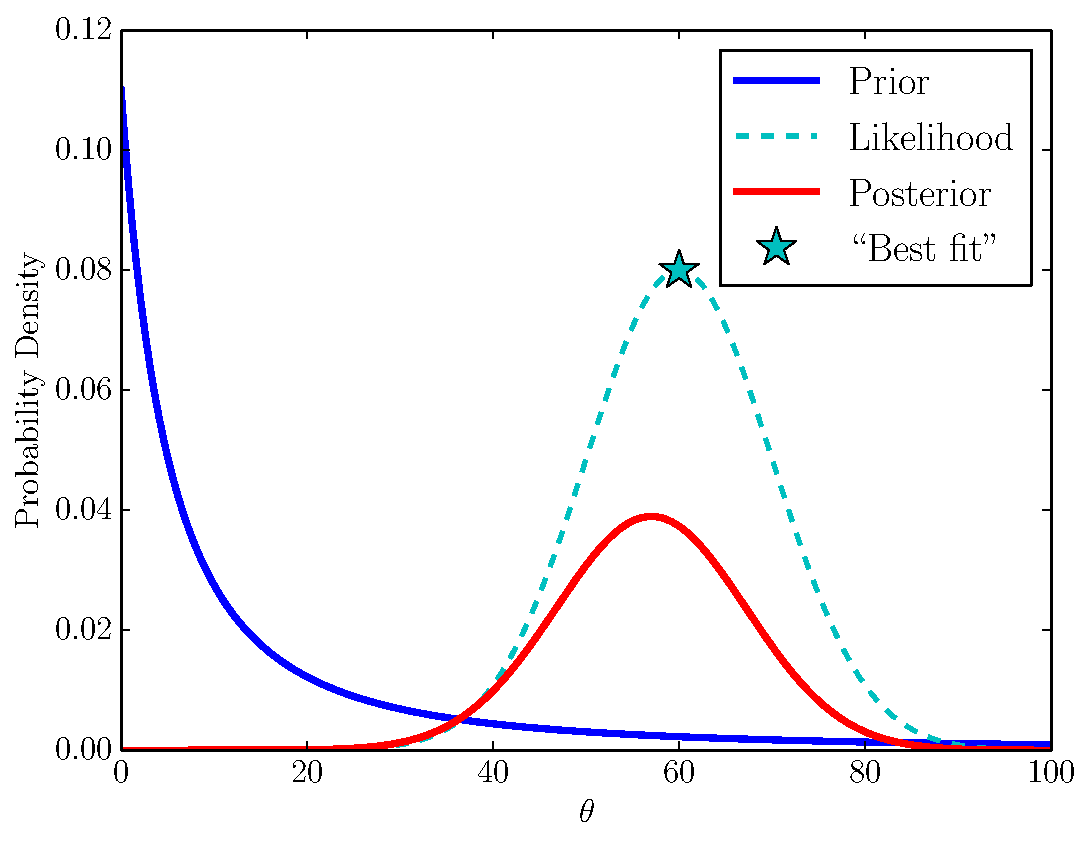
\includegraphics[scale=0.5]{bayes.pdf}
\caption{An example posterior distribution for a single parameter.
\label{fig:bayes}}
\end{center}
\end{figure}

\section{Transit Example}

The true curve, shown in red in Figure~\ref{fig:transit_data}, was given by:
\begin{eqnarray*}
\mu(t) &=& \left\{
\begin{array}{lr}
10, & 2.5 \leq t \leq 4.5\\
5,  & \textnormal{otherwise}.
\end{array}
\right.
\end{eqnarray*}

Let's assume that we didn't know this, but we did know the true curve
was a function of the following form:
\begin{eqnarray*}
\mu(t) &=& \left\{
\begin{array}{lr}
A, & (t_c - w/2) \leq t \leq (t_c + w/2)\\
A-b,  & \textnormal{otherwise}.
\end{array}
\right.
\end{eqnarray*}

We don't know the values of $A$, $b$, $t_c$, and $w$,
but we do know the data $D$. Applying Bayesian inference to this problem
involves calculating the posterior distribution for $A$, $b$, $t_c$, and $w$,
given the data $D$. For this specific setup, Bayes' rule states:

\begin{eqnarray}
p(A, b, t_c, w | D) &=& \frac{p(A, b, t_c, w)p(D | A, b, t_c, w)}{p(D)}
\end{eqnarray}

So, in order for the posterior distribution to be well defined, we need to
choose a prior distribution $p(A, b, t_c, w)$ for the parameters, and a
sampling distribution $p(D | A, b, t_c, w)$ for the data. Since the denominator
$p(D)$ is not a function of the parameters, it plays the role of a normalising
constant that ensures the posterior distribution integrates to 1, as any
probability distribution must.

\begin{figure}
\begin{center}
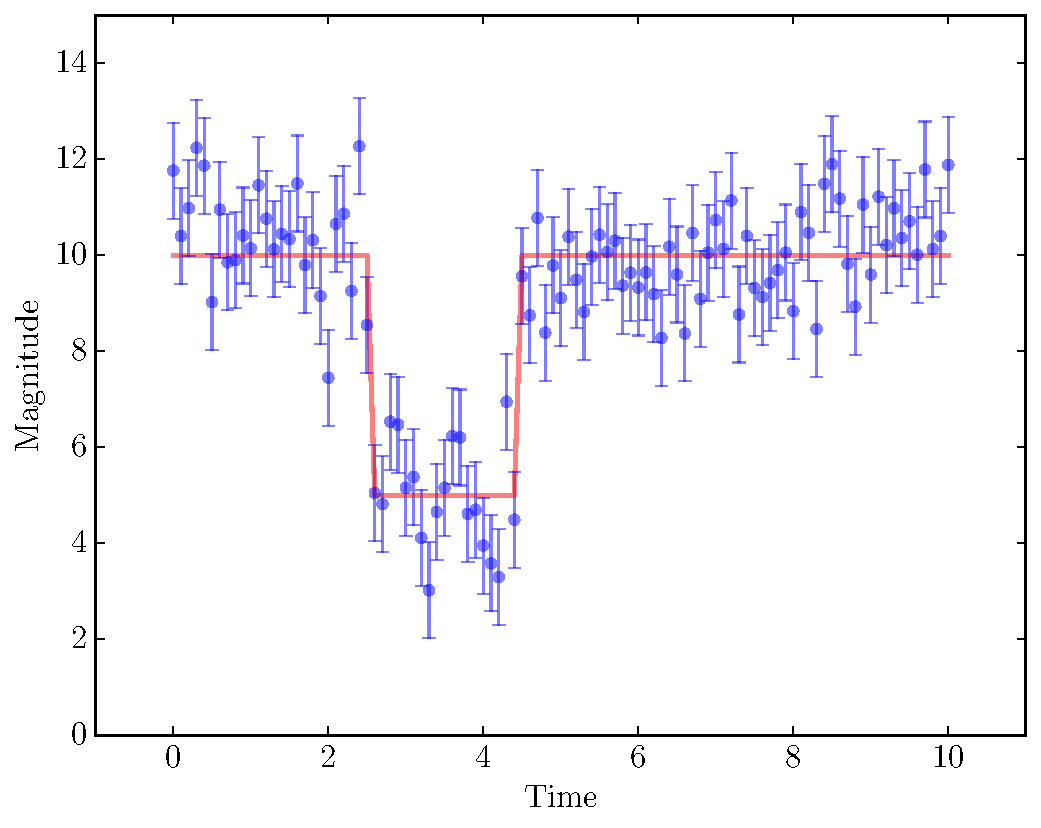
\includegraphics[scale=0.5]{../Code/transit_data.pdf}
\caption{The ``transit'' data set. The red curve shows the model prediction
based on the true values of the parameters.\label{fig:transit_data}}
\end{center}
\end{figure}

We want to know the values of the unknown parameters.
The {\it sampling distribution} is the probability distribution would assign
for the data, if we knew the true values of the parameters.
In many situations, it is conventional to assign a normal distribution
(also known as a gaussian distribution) to each data point, where the mean
of the normal distribution is the noise-free model prediction, and the
standard deviation of the normal distribution is given by the size of the
error bar. Later, we will see how to relax these assumptions.




\section{Assigning Prior Distributions}
It has been said ({\bf by whom?}) that there are only two open problems in
Bayesian inference. The first is how to assign prior distributions, and the
second is how to calculate the results.

It is sometimes said that there are two different kinds of Bayesian inference,
{\it subjective} and {\it objective}, with different methods for choosing
priors. My view is that Bayesian describes a {\it hypothetical}
state of prior knowledge, held by an idealised reasoner. When we apply
Bayesian inference, we are studying how the idealised reasoner would update
their state of knowledge based on the information we use in the calculation.

In many cases, we can just use simple ``default'' choices for the prior and
the sampling distribution (e.g. a uniform prior for a parameter, and a
``gaussian noise'' assumption for the data). A lot of analyses work just fine
with these assumptions. However, occasionally it makes sense to spend a lot of
time and effort thinking about the prior distributions. Some Bayesian statisticians, who are not
necessarily experts in the fields of their clients, conduct elaborate interviews
with experts to try and create a prior that models the experts' beliefs well.
This process is called {\it elicitation}.
For example, consider the Intergovernmental Panel on Climate Change (IPCC),
who periodically write immense reports summarising humanity's state of knowledge
about global warming.
Consider the question ``{\it How much will the global average temperature
increase in the next 100 years?}''. This is exactly the kind of situation where
elicitation of an expert's probabilities is very important: a lot is known,
and a lot is at stake. In this situation, it wouldn't be very wise to rely on
convenient ``vague'' priors!

\subsection{Probability distributions have consequences}
When you assign prior distributions, it is more easy than you might expect to
build in an assumption that you don't really agree with. To demonstrate this,
let's derive some consequences of the prior distributions we used in the
transit example.


\section{What is the data?}
It can sometimes be helpful to think carefully about exactly what your data set
contains, and whether it is all ``data'' in the sense of Bayesian inference.
In the transit example, we chose a sampling distribution for the data, but this
sampling distribution was for the $y$-values of the data
(the flux measurements). Note that we never assigned a probability distribution
for the {\it times} of the data points, even though we might think of that as
part of the data (it's probably in the same file as the measurements, after all).
In fact, because we didn't assign a probability distribution for it, the
timestamps were not data at all, but part of the prior information $I$.
Therefore, it is completely justifiable to use the timestamps when assigning
the prior and the sampling distribution.



\section{The Metropolis Algorithm}
The Metropolis-Hastings algorithm, also known as the Metropolis algorithm, is
the most fundamental MCMC algorithm. It is quite straightforward to implement,
and works well on most problems.

The version of the Metropolis algorithm presented here is sometimes called
{\it random walk} Metropolis, because of the choice of the proposal
distribution. More sophisticated choices are often possible, but usually
require problem-specific knowledge. Consider a problem with a single unknown
parameter $x$. If the prior is some density $\pi(x)$ and the likelihood
function is $\mathcal{L}(x)$, then the posterior distribution will be
proportional to $\pi(x)\mathcal{L}(x)$.

The ``random walk'' proposal generates a proposed value $x'$ from a normal
(gaussian) distribution centered around the current position $x$. The user
is free to choose the width of the normal distribution. Here is a Python code
snippet showing a proposal with width {\tt L}:

\begin{minted}[mathescape,
               numbersep=5pt,
               gobble=2,
               frame=lines,
               framesep=2mm]{python}
  # Generate a proposal
  proposal = x + L*rng.randn()
\end{minted}

The performance of the Metropolis algorithm seems to depend quite strongly on
the width of the proposal distribution. It's usually not a good idea to spend
a long time on preliminary runs to find an optimal width. Instead, I recommend
that you use a mixture of widths. Basically, every time we make a proposal,
the width is drawn from some range, rather than being constant.
\begin{minted}[mathescape,
               numbersep=5pt,
               gobble=2,
               frame=lines,
               framesep=2mm]{python}
  # A heavy-tailed proposal distribution
  # Generate a standard deviation
  L = 10.**(1.5 - 6.*rng.rand())

  # Use the standard deviation for the proposal
  proposal = x + L*rng.randn()
\end{minted}

With this proposal, the minimum width is
$10^{-4.5} \approx 3.16 \times 10^{-5}$, and the maximum width is
$10^{1.5} \approx 31.6$.

The effective proposal distribution is now very heavy-tailed.



\section{Birth and death moves}
Sometimes, when you are trying to fit a model to data, there is uncertainty
not just about the values of the model parameters, but also how many model
parameter exist in the first place. One example is
the radial velocity technique for detecting extra-solar planets
\citep{gregory}, where the goal is to fit a signal to a sparse data set, where
we don't know how many components (planets) there are.



\section{Model Selection and Nested Sampling}
Nested Sampling is a Monte Carlo algorithm introduced by \citet{skilling}.
Several variants of Nested Sampling exist, and most of them are somewhat
complicated. Here, I will present a simple version of Nested Sampling which
is sufficient to solve a wide range of problems. This approach is similar to
the one presented in the introductory textbook by \citet{sivia}.

Many more complex and sophisticated versions of
Nested Sampling exist, such as the popular MultiNest \citep{multinest},
my own Diffusive Nested Sampling \citep{dnest}, and several others. These
algorithms, while all based on the insights of \citet{skilling}, are very
different in detail. See the appendix for more details.

Consider two different models $M_1$ and $M_2$ which are mutually exclusive
(they can't both be true).
Suppose $M_1$ has parameters
$\btheta_1$, and $M_2$ has its own parameters $\btheta_2$. The methods
described previously can be used to calculate the posterior distribution for
$M_1$'s parameters:
\begin{eqnarray}
p(\btheta_1 | D, M_1) &=& \frac{p(\btheta_1 | M_1)p(D | \btheta_1, M_1)}
{p(D | M_1)}
\end{eqnarray}
You can also fit model $M_2$ to the data, i.e. get the posterior distribution
for $M_2$'s parameters:
\begin{eqnarray}
p(\btheta_2 | D, M_2) &=& \frac{p(\btheta_1 | M_2)p(D | \btheta_2, M_2)}
{p(D | M_2)}
\end{eqnarray}
This is all very well, but you might want to know whether $M_1$ or $M_2$ is
more plausible overall, given your data. That is, you want the posterior
probabilities $P(M_1 | D)$ and $P(M_2 | D)$.

In this situation, it's usually easier to calculate the ratio of the two
posterior probabilities, which is sometimes called the {\it posterior odds
ratio}:
\begin{eqnarray}
\frac{P(M_2 | D)}{P(M_1 | D)} &=& \frac{P(M_2)}{P(M_1)}
\times \frac{P(D | M_2)}{P(D | M_1)}
\end{eqnarray}

As you might expect, the posterior odds for $M_2$ over $M_1$ depends on the
prior odds: was $M_2$ more plausible than $M_1$ before taking into account the
data? The other ratio is a ratio of likelihoods, how probable was the data
assuming $M_2$ vs assuming $M_1$? These likelihoods aren't the likelihoods
for a specific value of the parameters, but instead likelihoods for the model
as a whole. To distinguish this kind of likelihood from the standard kind (which
is a function of the model parameters), the term {\it marginal likelihood} or
{\it evidence} is used. The marginal likelihood for $M_1$ is:
\begin{eqnarray}
p(D | M_1) &=& \int p(\btheta_1 | M_1) p(D | \btheta_1, M_1) \, d^{N_1} \btheta_1
\end{eqnarray}






%Bla bla bla \citep{lecturer1:abreu10}, \citep{lecturer1:abreu100}

%\input lecturer1/lecturer1.bbl

